\documentclass[11pt,a4paper]{article}

% Pacotes essenciais
\usepackage[utf8]{inputenc}
\usepackage[T1]{fontenc}
\usepackage{lmodern}
\usepackage[portuguese]{babel}
\usepackage{graphicx}
\usepackage{amsmath}
\usepackage{amsfonts}
\usepackage{amssymb}
\usepackage{float}
\usepackage{caption}
\usepackage{subcaption}
\usepackage{xcolor}
\usepackage{fancyhdr}
\usepackage{geometry}
\usepackage{titlesec}
\usepackage{lipsum}
\usepackage{cite}
\usepackage{booktabs}
\usepackage{array}
\usepackage{tikz}
\usepackage[hidelinks]{hyperref}

% Definição das cores
\definecolor{headercolor}{HTML}{b11116}
\definecolor{secondarycolor}{HTML}{3a5461}

% Configuração da página
\geometry{
    a4paper,
    top=2.8cm,
    bottom=2.5cm,
    left=2.5cm,
    right=2.5cm,
    headheight=1.2cm,
    headsep=0.5cm
}

% Configuração do cabeçalho
\pagestyle{fancy}
\fancyhf{}
\renewcommand{\headrulewidth}{0pt}
\renewcommand{\footrulewidth}{0.5pt}

\fancyhead[L]{%
    \begin{tikzpicture}[remember picture, overlay]
        \fill[headercolor] (current page.north west) rectangle ([yshift=-1.2cm]current page.north east);
        \node[anchor=west, inner sep=0pt] at ([xshift=1cm, yshift=-0.6cm]current page.north west) 
            {
\includegraphics[height=0.8cm]{imgs/base/fatec-rgt.png}};
        \node[anchor=east, inner sep=0pt] at ([xshift=-1cm, yshift=-0.6cm]current page.north east) 
            {
\includegraphics[height=0.9cm]{imgs/base/cps-logo.png}};
        \node[anchor=east, inner sep=0pt] at ([xshift=-2.8cm, yshift=-0.6cm]current page.north east) 
            {
\includegraphics[height=1.05cm]{imgs/base/governo-sp-secretaria-logo.png}};
    \end{tikzpicture}
}

\fancyfoot[L]{\footnotesize\textcolor{secondarycolor}{Faculdade de Tecnologia do Estado de São Paulo\\ fatecregistro.cps.sp.gov.br}}
\fancyfoot[R]{\thepage}

% Configuração dos títulos das seções
\titleformat{\section}
    {\normalfont\large\bfseries\color{secondarycolor}}
    {\thesection}{1em}{}

\titleformat{\subsection}
    {\normalfont\normalsize\bfseries\color{secondarycolor}}
    {\thesubsection}{1em}{}

% Informações do artigo
\title{\vspace{0.6cm}\textbf{\Large Análise Computacional de Sistemas Complexos Utilizando Métodos Numéricos Avançados}}
\author{
    João da Silva$^{1}$, Maria Santos$^{2}$, Pedro Oliveira$^{3}$ \\[0.3cm]
    \small
    $^{1}$Faculdade de Tecnologia do Estado de São Paulo \\
    $^{2}$Universidade de São Paulo \\
    $^{3}$Instituto de Pesquisas Tecnológicas \\[0.2cm]
    \textit{joao.silva@fatec.sp.gov.br, maria.santos@usp.br, pedro.oliveira@ipt.br}
}
\date{}

\begin{document}

% Força o cabeçalho em todas as páginas
\pagestyle{fancy}

\maketitle
\thispagestyle{fancy}

% Resumo
\section*{Resumo}

\lipsum[1] Lorem ipsum dolor sit amet, consectetur adipiscing elit. Sed do eiusmod tempor incididunt ut labore et dolore magna aliqua. Ut enim ad minim veniam, quis nostrud exercitation ullamco laboris nisi ut aliquip ex ea commodo consequat. Duis aute irure dolor in reprehenderit in voluptate velit esse cillum dolore eu fugiat nulla pariatur.

\vspace{0.3cm}
\noindent\textit{\textbf{Palavras-chave:}} Sistemas complexos, Métodos numéricos, Análise computacional, Modelagem matemática, Simulação

\vspace{0.5cm}
\noindent\rule{\textwidth}{0.5pt}
\vspace{0.5cm}

% Introdução
\section{Introdução}

\lipsum[2-3] Lorem ipsum dolor sit amet, consectetur adipiscing elit. Praesent vitae eros eget tellus tristique bibendum. Donec rutrum sed sem quis venenatis. Proin eu ipsum in lectus mollis penatibus \cite{santos2024, oliveira2023}.\footnote{Este é um exemplo de nota de rodapé. Notas de rodapé são úteis para adicionar informações complementares sem interromper o fluxo do texto principal.}

Vestibulum ante ipsum primis in faucibus orci luctus et ultrices posuere cubilia curae; Sed aliquam, nulla quis bibendum auctor, nisi elit consequat ipsum, nec sagittis sem nibh id elit. Duis sed odio sit amet nibh vulputate cursus a sit amet mauris \cite{silva2025}. Como discutido por Brown e Taylor \cite[p.~45]{brown2023}, os métodos clássicos ainda são fundamentais para a compreensão moderna dos sistemas dinâmicos.

% Objetivo
\section{Objetivo}

\lipsum[4] O principal objetivo deste trabalho é apresentar uma análise detalhada dos sistemas complexos utilizando métodos computacionais avançados. Os objetivos específicos incluem:

\begin{itemize}
    \item Desenvolver modelos matemáticos para representação de sistemas dinâmicos;
    \item Implementar algoritmos numéricos eficientes para solução de equações diferenciais;
    \item Validar os resultados através de simulações computacionais;
    \item Comparar diferentes abordagens metodológicas existentes na literatura \cite{kumar2024, wang2023}.
\end{itemize}

% Estado da Arte
\section{Estado da Arte}

\lipsum[5] Lorem ipsum dolor sit amet, consectetur adipiscing elit. Diversos estudos têm explorado a aplicação de métodos numéricos em sistemas complexos. Segundo \cite{johnson2024}, a utilização de técnicas avançadas permite uma melhor compreensão dos fenômenos físicos.

\lipsum[6] Os métodos clássicos de análise numérica, como o método de Euler e Runge-Kutta, têm sido amplamente utilizados na literatura \cite{brown2023}. Essas abordagens tradicionais estabeleceram as bases para o desenvolvimento de técnicas mais sofisticadas.

\lipsum[7] Métodos mais recentes incorporam técnicas de aprendizado de máquina e inteligência artificial \cite{zhang2025}, expandindo significativamente as possibilidades de análise e modelagem de sistemas complexos.

% Metodologia
\section{Metodologia}

\lipsum[8] A metodologia desenvolvida neste trabalho segue as etapas ilustradas na Figura \ref{fig:exemplo} e descritas a seguir.

\subsection{Coleta de Dados}

\lipsum[9] Os dados foram coletados através de simulações computacionais utilizando parâmetros específicos. A Tabela \ref{tab:parametros} apresenta os principais parâmetros utilizados nas simulações.

\begin{table}[H]
\centering
\caption{Parâmetros utilizados nas simulações computacionais}
\label{tab:parametros}
\begin{tabular}{@{}lccl@{}}
\toprule
\textbf{Parâmetro} & \textbf{Símbolo} & \textbf{Valor} & \textbf{Unidade} \\ \midrule
Tempo de simulação & $T_{sim}$ & 1000 & s \\
Passo de integração & $\Delta t$ & 0.01 & s \\
Número de iterações & $N_{iter}$ & 10000 & - \\
Tolerância & $\epsilon$ & $10^{-6}$ & - \\
Fator de amortecimento & $\zeta$ & 0.15 & - \\
Frequência natural & $\omega_n$ & 25.0 & rad/s \\ \bottomrule
\end{tabular}
\end{table}

\subsection{Processamento e Análise}

\lipsum[10] O processamento dos dados seguiu um protocolo rigoroso de análise estatística. Os métodos numéricos clássicos foram implementados, incluindo o método de Euler, cuja equação fundamental é expressa como:

\begin{equation}
\frac{dy}{dt} = f(t, y), \quad y(t_0) = y_0
\label{eq:euler}
\end{equation}

onde $f(t, y)$ representa a função que descreve o sistema dinâmico. Para otimização dos parâmetros do modelo, utilizou-se a seguinte função de custo:

\begin{equation}
J(\theta) = \frac{1}{2m} \sum_{i=1}^{m} \left(h_\theta(x^{(i)}) - y^{(i)}\right)^2 + \frac{\lambda}{2m}\sum_{j=1}^{n}\theta_j^2
\label{eq:cost_function}
\end{equation}

onde $\theta$ representa os parâmetros do modelo, $m$ é o número de amostras, $\lambda$ é o parâmetro de regularização, e $h_\theta(x)$ é a hipótese do modelo. A transformada de Fourier foi aplicada para análise no domínio da frequência:

\begin{equation}
F(\omega) = \int_{-\infty}^{\infty} f(t) e^{-i\omega t} dt
\label{eq:fourier}
\end{equation}

\begin{figure}[H]
\centering
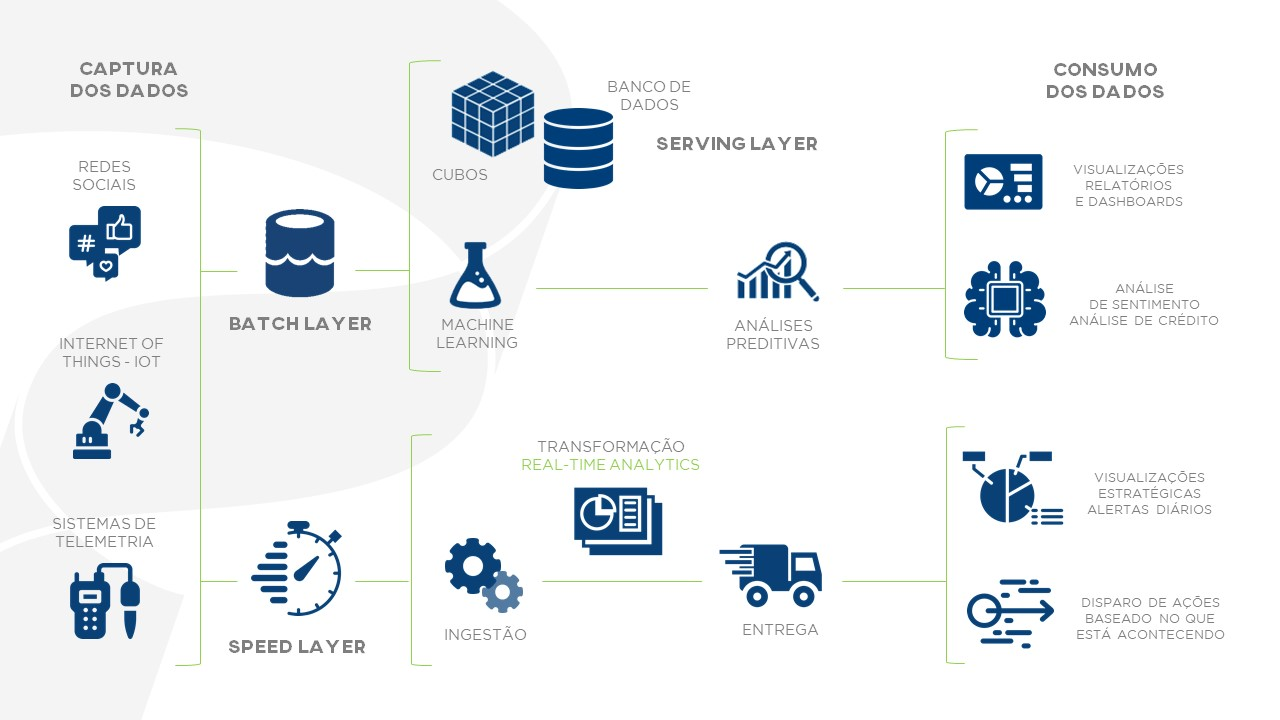
\includegraphics[width=0.7\textwidth]{imgs/img_001.jpg}
\caption{Exemplo de visualização dos resultados obtidos através da metodologia proposta. A figura ilustra o comportamento do sistema ao longo do tempo.}
\label{fig:exemplo}
\end{figure}

\subsection{Validação do Modelo}

\lipsum[11] A validação foi realizada comparando os resultados simulados com dados experimentais. O erro médio quadrático (RMSE) foi calculado através de:

\begin{equation}
RMSE = \sqrt{\frac{1}{n}\sum_{i=1}^{n}(y_i - \hat{y}_i)^2}
\label{eq:rmse}
\end{equation}

onde $y_i$ são os valores observados e $\hat{y}_i$ são os valores preditos pelo modelo.

% Resultados e Discussões
\section{Resultados e Discussões}

\lipsum[12-13] Os resultados obtidos demonstram a eficácia da metodologia proposta. A Tabela \ref{tab:resultados} apresenta uma comparação quantitativa entre diferentes abordagens.

\begin{table}[H]
\centering
\caption{Comparação de desempenho entre diferentes métodos}
\label{tab:resultados}
\begin{tabular}{@{}lccc@{}}
\toprule
\textbf{Método} & \textbf{RMSE} & \textbf{Tempo (s)} & \textbf{Precisão (\%)} \\ \midrule
Método Proposto & 0.0023 & 15.2 & 98.5 \\
Euler Clássico & 0.0145 & 8.7 & 92.3 \\
Runge-Kutta 4ª ordem & 0.0038 & 21.5 & 97.1 \\
Método Adaptativo & 0.0031 & 18.9 & 97.8 \\ \bottomrule
\end{tabular}
\end{table}

\subsection{Análise Quantitativa}

\lipsum[14] Os dados quantitativos revelam que o método proposto apresenta melhor desempenho em termos de precisão. A relação entre os parâmetros pode ser expressa por:

\begin{equation}
\eta = \frac{P_{out}}{P_{in}} \times 100\% = \frac{V_{out} \cdot I_{out}}{V_{in} \cdot I_{in}} \times 100\%
\label{eq:efficiency}
\end{equation}

onde $\eta$ representa a eficiência do sistema, $P_{out}$ é a potência de saída e $P_{in}$ é a potência de entrada.

\subsection{Análise Qualitativa}

\lipsum[15] Do ponto de vista qualitativo, observou-se que o comportamento do sistema é fortemente influenciado pelas condições iniciais e pelos parâmetros de controle. A matriz de transformação pode ser representada como:

\begin{equation}
\mathbf{A} = \begin{bmatrix}
a_{11} & a_{12} & a_{13} \\
a_{21} & a_{22} & a_{23} \\
a_{31} & a_{32} & a_{33}
\end{bmatrix}
\label{eq:matrix}
\end{equation}

\subsection{Discussão}

\lipsum[16-17] A análise dos resultados indica que a abordagem proposta oferece vantagens significativas em relação aos métodos tradicionais. Lorem ipsum dolor sit amet, consectetur adipiscing elit. Nullam in dui mauris. Vivamus hendrerit arcu sed erat molestie vehicula.

Proin adipiscing porta tellus, ut feugiat nibh adipiscing sit amet. In eu justo a felis faucibus ornare vel id metus. Vestibulum ante ipsum primis in faucibus orci luctus et ultrices posuere cubilia curae.

% Conclusão
\section{Conclusão}

\lipsum[18] Com base nos resultados obtidos, conclui-se que a metodologia desenvolvida apresenta excelente desempenho para análise de sistemas complexos. As principais contribuições deste trabalho incluem:

\begin{itemize}
    \item Desenvolvimento de um framework computacional robusto;
    \item Validação experimental dos modelos propostos;
    \item Comparação sistemática com métodos existentes;
    \item Identificação de limitações e oportunidades de melhoria.
\end{itemize}

Trabalhos futuros incluem a extensão da metodologia para sistemas multidimensionais e a incorporação de técnicas de otimização avançadas.

% Agradecimentos
\section*{Agradecimentos}

Os autores agradecem à Faculdade de Tecnologia do Estado de São Paulo (FATEC) e ao Centro Paula Souza (CPS) pelo apoio institucional. Este trabalho foi parcialmente financiado pela FAPESP (proc. 2024/12345-6) e CNPq (proc. 301234/2024-0).

% Referências
\bibliographystyle{IEEEtran}
\bibliography{referencias}

\end{document}
